% introduction
\begin{frame}{Citations and Bibliographies}{Introduction}
\textbf{Bibliography} - a list of the books referred to in a scholarly work,
typically printed as an appendix.  \\ \vspace{1em}

\footnotesize
When it comes to bibliography-management packages, there are three main options
in LaTeX: bibtex, natbib and biblatex. BibTex LaTeX has its own bibliography format
\texttt{.bib}, that you can find almost everywhere and is mostly compatible
with above listed packages.

It is possible to write citations manually, but when they are large in number,
it is faster to automate it. \vspace{2em}

\begin{columns}
    \begin{column}{0.4\textwidth}
        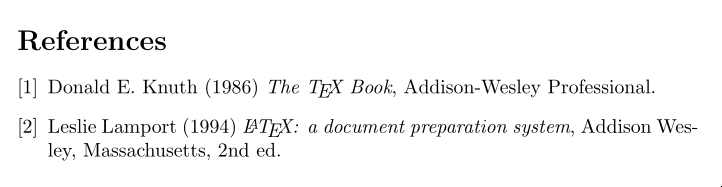
\includegraphics[width=\textwidth]{bib1.png}
    \end{column}
    \begin{column}{0.6\textwidth}
        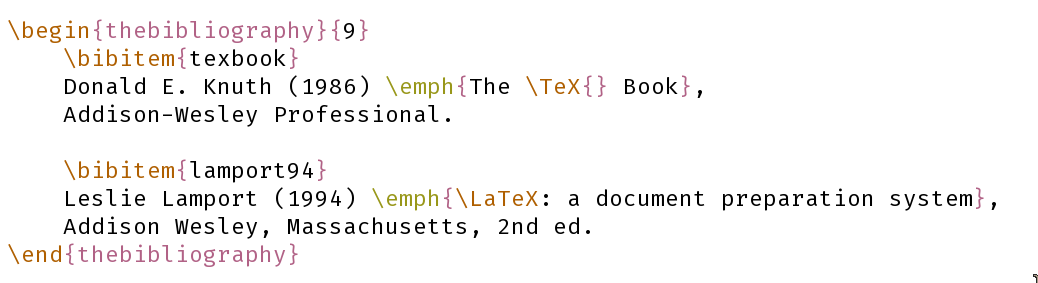
\includegraphics[width=\textwidth]{bib1_code.png}
    \end{column}
\end{columns}
\end{frame}


% bibtex
\begin{frame}[fragile]{Citations and Bibliographies}{BibTex}
\footnotesize
BibTex is built into \LaTeX and there is no need to use any other package.
\vspace{1em}

\begin{columns}
    \begin{column}{0.3\textwidth}
        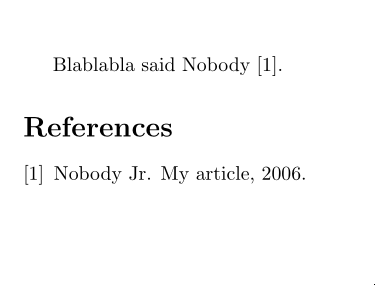
\includegraphics[width=\textwidth]{bib2.png}
    \end{column}
    \begin{column}{0.7\textwidth}
        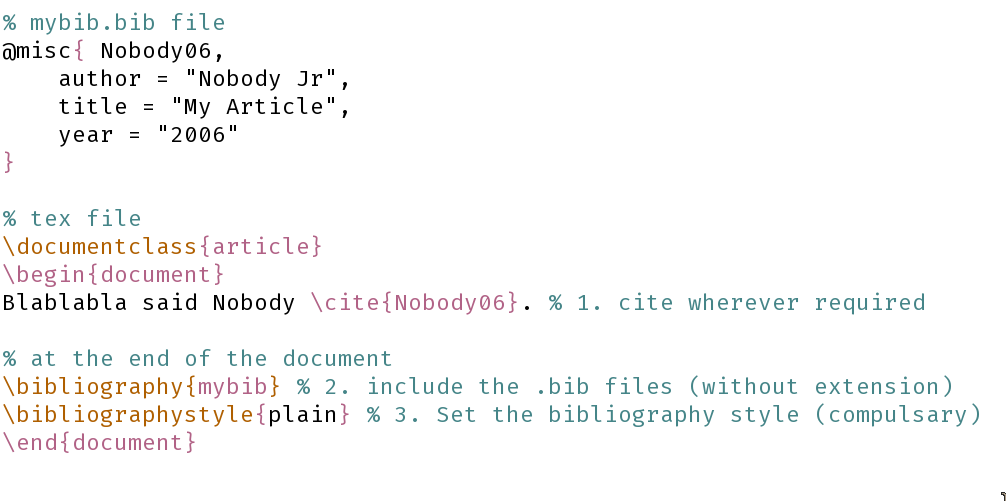
\includegraphics[width=\textwidth]{bib2_code.png}
    \end{column}
\end{columns}

Compiling in terminal takes a few extra steps, if a .bib file is used:
\tiny
\begin{lstlisting}
$ pdflatex myarticle.tex   # unresolved citations written to .aux
$ bibtex myarticle         # generata .bbl file from .aux file
$ pdflatex myarticle.tex   # resolves cross-references and adds citations
$ pdflatex myarticle.tex   # to make sure all entries are resolved and updated
\end{lstlisting}

\end{frame}

% task
\begin{frame}{Citations and Bibliographies}{Task-3}
Try solving the task 3. The solution is...\\ \pause
\vspace{1em}
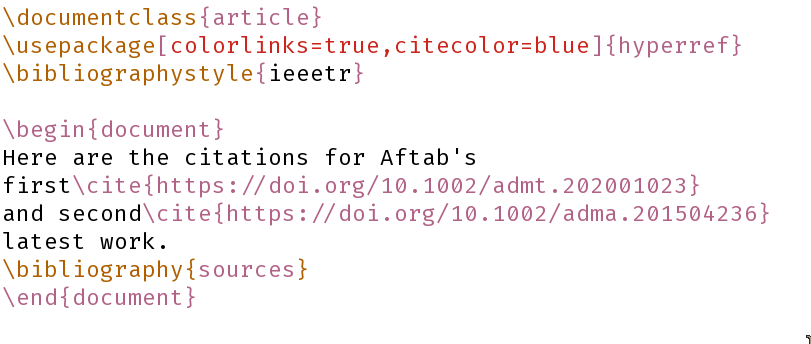
\includegraphics[width=\textwidth]{3.png}
You can find the sources.bib file renamed to `h` in the `test3`
directory.
\end{frame}
